\section{Experimental Setup}
\label{sec:setup}
\textbf{v1.} Seven OpenRouter models (October 2026; router defaults; listed
in Table~\ref{tab:models}) ran on 20 tasks (10 effect, 10 null) with 3 repeats in
\cfg{Ref}, \cfg{Leak}, \cfg{Silent}, and \cfg{Stale}, for 1,680 runs and
\$35.60. \cfg{Prov} regrades the 420 \cfg{Ref} traces. We re-analyze these
records without new calls and re-execute all 1,665 cited confirmation scripts
under instrumentation; every re-execution reproduced its recorded output.
\textbf{v2.} Forty new tasks (seeds 5000--5039, 20 effect and 20 null) come
from the unchanged generator and are frozen with SHA-256 manifests. Four v1
models (GPT-6.1-sol, Haiku 5.5, GPT-6-luna, DeepSeek-V4.1-flash; same
snapshots) ran once per task in \cfg{Ref}, \cfg{Sep\_read}, \cfg{Int\_mask},
and \cfg{Fresh\_cache}, for 640 runs and \$2.94. Endpoints were pinned, reasoning effort was \texttt{low}, and condition
order was randomized within blocks (Appendix~\ref{app:repro}). A deterministic \emph{reference agent} screens
all ten exposures with the oracle model on exploration data, locks the
minimum-$p$ exposure, confirms once, and submits the implied decision.

\section{Results}
\label{sec:results}

\begin{figure}[t]
  \centering
  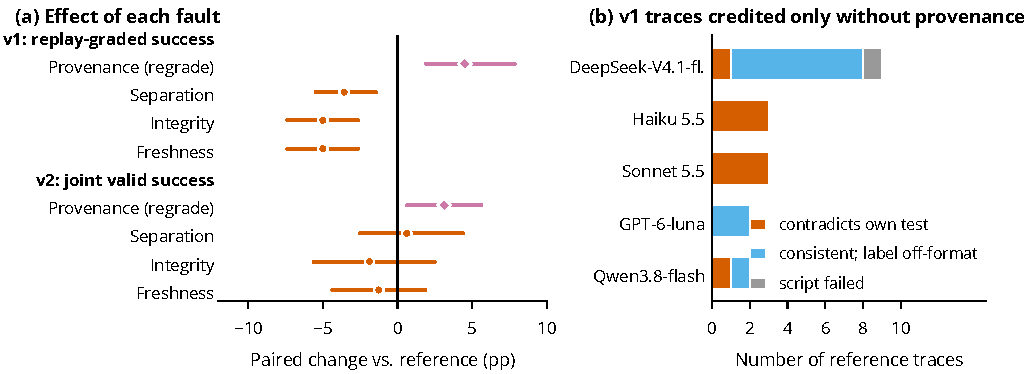
\includegraphics[width=\linewidth]{figures/fig_effects.pdf}
  \caption{\textbf{(a)} Paired change vs.\ the reference pipeline with 95\%
  task-cluster bootstrap intervals. Diamonds regrade identical traces (change in
  credit); circles are fresh runs. v1 and v2 use different success
constructs, so magnitudes are not comparable across blocks. \textbf{(b)} The 19
  v1 reference traces credited only by the answer-only grader, by what the
  agent's own confirmation output showed. Full table: Appendix~\ref{app:results}.}
  \label{fig:effects}
\end{figure}

\subsection{Truth and evidence diverge in both directions}
\label{sec:diverge}
Applying the oracle to every recoverable hypothesis in the 420 v1 reference
traces gives 271 conclusions that are true and supported, 30 that are
\emph{supported but false} (29 false discoveries with held-out $p<0.05$ and
one missed effect), and only 1 that is true but unsupported. Another 118 have
no evidential status because no single hypothesis was locked
(Appendix Figure~\ref{fig:tec}). The v1 reference grade is therefore \emph{replay-graded}, not the v2
construct: of its 364 credits, 262 are true and oracle-supported, 63
undetermined, 38 null-task abstentions, and 1 unsupported. The supported-but-false cell is concentrated in particular
datasets. Of 116 v1
false discoveries, 114 fall on two null tasks whose confirmation split
contains an oracle-significant exposure, and the deterministic reference agent
also errs on both (Appendix~\ref{app:dgp-null}). Excluding them lowers the
null false-discovery rate from 13.8\% to 0.3\%. On fresh simulated data the
reference agent's rate is 4.8\% (95\% CI 4.3--5.5). The 13.8\% therefore
describes which 10 null datasets were drawn, each re-sampled 84 times; it is
not agent calibration, although agents' selection policies still decide
whether such associations get found and reported (\S\ref{sec:multitest}). In v2, all 3 false discoveries in 80 null reference
runs fall on the one task where the reference agent also errs.
\emph{Lesson: report false discoveries against a trusted baseline on the same
datasets, and count datasets, not runs.}

\subsection{What an answer-only grader credits}
\label{sec:prov}
Dropping the evidence check from the v1 grader raises credit on identical
traces by $+4.5$ pp ($[+1.9,+7.9]$). The sign is fixed by construction, so
the content is the composition (Figure~\ref{fig:effects}b).
\textbf{Eight traces contradict their own evidence.} The confirmation
printed a significant exposure, and the agent submitted ``none'' or
``inconclusive'' on a null task. In Sonnet's case it cited a sign reversal
from exploration, a defensible judgment outside the stated rule that was right
only because the truth was null.
\textbf{Ten are correct readings of non-significant tests that
broke the output contract.} The instructions defined \texttt{answer} as the
conclusion, but these scripts used it to name the tested candidate. A typical
DeepSeek script printed \texttt{\{"answer":"nitrate", "p\_value":0.2015\}},
and the agent submitted ``none''. The label check rejected a decision that its
own evidence supports. \textbf{One} has a failed script.
So 2.6 of the 4.5 pp reflects format compliance, not evidence violations
(Appendix~\ref{app:labels}); 8 of these 11 are DeepSeek's, and without
DeepSeek the estimate is $+2.8$ pp.
v2 removes the label problem, because decisions cite records, but
\cfg{Prov\_grade} still adds $+3.1$ pp ($[+0.6,+5.6]$). All 5 newly credited
runs are Haiku declaring ``no confirmed discovery'' on null tasks without
calling \texttt{confirm}, because exploration showed nothing worth testing
(Appendix~\ref{app:traces}). This lifts Haiku from last to first of four
models, though on 5 runs of one model and in only 64\% of bootstrap
replicates.
\emph{Lesson: when half the tasks are null, ``no discovery'' is free unless
credit requires evidence.}

\subsection{One confirmation call is not one test}
\label{sec:multitest}
The v1 harness enforced one \texttt{confirm} \emph{call}, but each call
executed arbitrary code on the confirmation split. Several distinct
quantities collapse under ``confirm once'': the number of calls, the number
of candidates entering fitted models, the number of separate inferential
tests, whether the reported candidate was chosen \emph{using} confirmation
results, and whether a target was fixed beforehand. Logging every
\texttt{statsmodels}/SciPy fit inside the re-executed scripts recovers the
second and third directly (Algorithm~\ref{alg:recover}). Among the 1,665
scripts (Appendix Table~\ref{tab:taxonomy}), 56.2\% fit one candidate,
31.4\% fit several candidates in one model structure (typically all ten as
joint regressors), 10.9\% fit separate models to different candidates, and
1.6\% have no identifiable fit.
These are different statistical acts. A joint regression may still serve a
single pre-specified coefficient, but separate fits are a screen on held-out
data. In 46 of the 47 discoveries from separate-fit scripts, the reported
exposure was the smallest-$p$ candidate, and 18 of the 47 were false. 126 of the 182 separate-fit scripts contain a correction pattern such as
Bonferroni; this is a lexical indicator, not a verified procedure, and the
reported $p$ was typically uncorrected. Locking a hypothesis on exploration data and testing it once
discovers on 4.8\% of nulls. Taking the minimum $p$ over ten confirmation
tests discovers on 39.4\%, close to $1-0.95^{10}=40.1\%$ for independent tests.

Single-test scripts matched the oracle's significance call in 793 of 794
cases: the arithmetic was right, but the mapping from tool call to
inferential act was not fixed. v2 fixes it, since \texttt{confirm} takes a
name, runs one test, and locks the hypothesis. Under v2, every confirmed
decision equalled the decision its record implied, against 8 contradictions
among v1 reference traces. Agents agreed with the deterministic reference
agent on 99.4\% of decisions and 95\% of locked hypotheses. Its 11 supported-but-false reference runs are sampling and selection error,
which no interface removes. \emph{Lesson: pre-registration must constrain the hypothesis and the
analysis, not the number of tool invocations.}

\subsection{Environment faults matter only when they manifest}
\label{sec:env}
\textbf{Observed effects.} In v1, replay-graded success fell by 3.6 pp under
\cfg{Leak} ($[-5.5,-1.4]$), 5.0 pp under \cfg{Silent} ($[-7.4,-2.6]$), and
5.0 pp under \cfg{Stale} ($[-7.4,-2.6]$).
Holm-adjusted task-level sign-flip randomization tests give $p=0.023$,
$0.006$, and $0.006$. All three keep their sign under every leave-one-task-out
refit and after removing the two dominant null tasks. Measured and replay-graded success
moved together (within 0.3 pp); replay agreement does not, however,
establish independent evidential validity.
The losses are concentrated: Qwen lost up to 21.7 pp and DeepSeek up to
16.7 pp, while GPT-6.1-sol, Sonnet, Gemini, and Haiku moved by at most 3.3 pp
(Appendix~\ref{app:sens}).

\textbf{Replay.} Re-executing the 420 reference action sequences unchanged in
each faulted environment moved the grade by 0, 0, and $-0.5$ pp. This holds
even though 26.7\% of the sequences contained an error that \cfg{Silent}
would hide and 42.1\% hit a stale entry under \cfg{Stale}. A fault changes the
grade of fixed behaviour only if it touches the cited confirmation, which
happened in 2 of 420 replays. The fresh-run losses are not mechanical. They are consistent with agents
responding to altered observations, but the comparisons do not identify the
mechanism; one Qwen trace shows such a response (Appendix~\ref{app:replay-trace}).

\textbf{Manifestation.} A scheduled fault is not a delivered treatment: masking
needs a failing run, and staleness needs two scripts sharing a key prefix. v2
agents used about six tool calls per run, so a masked failure reached the agent in 15\% of \cfg{Int\_mask} runs and a
stale output in 19\% of \cfg{Fresh\_cache} runs. The corresponding v1 rates
were 28\% and 44\%, under broader fault semantics. The held-out file was
visible in 88\% of \cfg{Sep\_read} runs but read in 4\%, never before the
lock.

\textbf{Scope of inference.} The v2 contrasts are $+0.6$, $-1.9$, and $-1.3$
pp, each with an interval of about $\pm4$ pp that includes zero (Holm
$p\ge0.56$). Runs in
which a v2 fault manifested reached 83\% (masked) and 80\% (stale) joint
validity, against 89\% and 91\% elsewhere. Manifestation is post-treatment
behaviour, however, so these contrasts are descriptive (Appendix~\ref{app:faults-cond}).
v1 and v2 differ in fault semantics, model panel, inference settings,
repeats, and tasks, so the smaller v2 effects cannot be attributed to the
trusted protocol (Appendix~\ref{app:faults-compare}). \emph{Lesson: an injected
defect is a treatment only to the extent that it reaches the agent. Report
trigger, visibility, and use with every fault effect.}

\section{Discussion}
\label{sec:discussion}
\textbf{Scientific truth does not validate scientific process.} Among v1
reference traces, 30 conclusions were supported and false, and 8 were true
but contradicted their own evidence. Agreement with the generating process
alone cannot separate a well-run non-replication from a lucky guess.
Benchmarks should report \fld{truth} and \fld{evid} separately and judge false
discoveries against a trusted agent run on the same datasets.

\textbf{Grader strictness is not grader correctness.} 11 of the v1 grader's
21 rejections in \cfg{Ref} were decisions consistent with a non-significant
test whose \texttt{answer} field named the tested candidate. The check
enforced format under the name of evidence, and the answer-only grader erred
the other way. A grader must encode the decision rule, as v2 does with typed
decisions and record lookup.

\textbf{Infrastructure defines the measured capability.} Under unrestricted
confirmation, correct inference, a screen of held-out data, and a lucky answer
earn the same score. A v2 score certifies hypothesis selection and decision
discipline, not statistical programming (Appendix~\ref{app:validity}).

\textbf{Limitations.} The results come from one linear-inference family, 20
(v1) and 40 (v2) datasets, four v2 models with one repeat, and one
implementation per fault. v1 used router defaults, and its sandbox let 2 of
1,680 runs read the held-out file (Appendix~\ref{app:validity}).

\section{Conclusion}
\label{sec:conclusion}
A
label-matching evidence check penalized correct inference, an answer-only
grader rewarded untested null decisions, and one call permitted many
tests. Fault effects depended on exposure; false discoveries concentrated
in particular datasets. A defensible scientific-agent pipeline executes the
confirmatory analysis itself, binds each decision to an immutable evidence
record, and reports truth, evidential support, and credit as distinct
quantities.
